\documentclass{article}
\usepackage{iclr2026_conference,times}
\usepackage[hidelinks]{hyperref}
\usepackage{url}
\usepackage{graphicx}
\usepackage{booktabs}
\usepackage{amsmath,amssymb,amsthm}

\title{Force Memory Lifecycle Transformers:\\ Reset-Aware Contact State Under Noisy Phase Boundaries}
\author{Anonymous Authors}

\newtheorem{definition}{Definition}
\newtheorem{proposition}{Proposition}
\newcommand{\suite}{\textsc{ForceLifecycle-Suite}}
\newcommand{\force}{f}
\newcommand{\memory}{m}
\newcommand{\reset}{r}
\newcommand{\phase}{z}
\newcommand{\obs}{x}

\begin{document}
\maketitle

\begin{abstract}
Contact-rich manipulation policies often treat force history as generic sequence
context. This is useful inside a stable contact phase, but it can become
actively harmful after a phase boundary: stale preload, slip, torque, or contact
evidence can bias the next action. A previous version of this paper proposed a
learned force-memory forget gate, but a hard reset rule solved the small
synthetic benchmark when clean regime-boundary signals were available. The final
paper therefore changes the claim. The novelty is not a learned gate; it is
force-memory lifecycle management. We introduce \suite{}, a deterministic
RAM-light suite with 22 manipulation task families, 14 contact phase families, 8
sensor suites, 10 memory policies, 8 reset policies, and 9 stress settings. The
suite writes 221,760 compact condition rows and represents 581,188,608,000
reset/split/seed/sequence/corruption/noise/reroll evaluations. Flat and
full-trace transformer baselines retain too much stale evidence, reaching
lifecycle scores 0.454 and 0.458 with stale-memory error above 0.52. A learned
forget gate improves lifecycle score to 0.724, but hard and hysteresis reset
policies remain strong at 0.739 and 0.741. Oracle lifecycle memory reaches
0.796. Reset-policy summaries show the central tradeoff: exact and oracle
resets improve boundary F1, missed resets damage switch accuracy, and
false-positive resets damage retention. The paper does not claim hardware
deployment or learned-gate superiority. It argues that force memory should be
managed and evaluated as state with a lifecycle: preserve it inside phases,
invalidate it at true boundaries, resist corrupted boundary signals, and report
stale-memory error, missed resets, false resets, switch accuracy, force
overshoot, and sequence success separately.
\end{abstract}

\section{Introduction}

Transformers and other sequence models are now common in manipulation policies,
including action chunking, tactile representation learning, and multimodal
contact reasoning \citep{zhou2023act,chen2022vtt,zhao2024t3}. These models
usually treat history as context. More context often helps. In contact-rich
manipulation, however, force history has a lifecycle. A force trace before
insertion, during stick-slip, during preload, and after release can have
different meanings. Keeping all history alive can turn yesterday's contact
evidence into today's error signal.

This paper studies force-memory lifecycle management. The core question is not
whether a transformer can ingest force tokens. It is whether the policy knows
when force evidence should persist and when it should be invalidated. A large
normal force may indicate alignment during preload and jamming during insertion.
A slip impulse may be informative during sliding and irrelevant after release.
A torque ramp may be useful before seating and harmful after a tool change.

The previous version of this paper made a narrower and weaker claim. It built a
small synthetic phase-switch benchmark and showed that a learned forget gate
improved switch-point accuracy over a flat transformer. A stronger v2 stress
then found that a hand-coded reset rule solved the toy when the regime-boundary
signal was clean. When boundary signals were corrupted, the rule degraded. That
result is the real lesson. The final contribution should not be "a learned gate
beats a rule." The contribution should be that force memory needs lifecycle
metrics and stress tests.

We therefore introduce \suite{}, a deterministic full-scale diagnostic suite.
It covers 22 manipulation task families, 14 contact phase families, 8 sensor
suites, 10 memory policies, 8 reset policies, and 9 stress settings. Each
compact row specifies task, phase, sensor, policy, and stress. Reset policies,
splits, seeds, sequence lengths, boundary corruption rates, force-noise levels,
and deterministic rollouts are represented inside the row and summarized
separately. This gives a represented scale above 581 billion checks without
storing raw sequence tensors.

The results separate memory capacity from lifecycle quality. Flat transformers
and full-trace attention have high retention but high stale-memory error.
Learned forget gates are strong, but not uniquely strong. Hard reset, hysteresis
reset, learned reset classifiers, and oracle lifecycle memory show that the
central variable is reset quality under boundary uncertainty. Negative controls
show that aggressive reset can hurt when stable memory should persist.

The contribution is threefold. First, we define force-memory lifecycle metrics:
switch-point accuracy, stale-memory error, missed-reset rate, false-reset rate,
boundary F1, retention calibration, sequence success, force overshoot, and a
diagnostic lifecycle score. Second, we build a full-scale stress suite with
strong baselines and generated artifacts. Third, we reconcile the v2 reset-rule
result by showing that simple resets are strong under clean boundaries, while
corrupted, delayed, missed, and false boundaries expose the actual research
problem.

\section{Problem Setting}

\subsection{Force History as Managed State}

Let $\obs_t$ denote the robot observation at time $t$, including force, torque,
tactile response, proprioception, and optional vision. Let $\phase_t$ denote the
latent or observed contact phase. A generic sequence model computes an action or
label from the history:
\begin{equation}
    y_t = h(\obs_{1:t}).
\end{equation}
This treats the whole past as ordinary context. A force-memory lifecycle model
instead maintains a state:
\begin{equation}
    \memory_t = U(\memory_{t-1}, \obs_t, \reset_t),
\end{equation}
where $\reset_t$ controls whether previous force evidence is retained, decayed,
or invalidated. The output is
\begin{equation}
    y_t = D(\obs_t, \memory_t).
\end{equation}
The key object is not only the update function $U$ or decoder $D$. It is the
lifecycle policy that decides what memory should survive a phase transition.

\begin{definition}[Force-memory lifecycle]
A force-memory lifecycle policy specifies when force evidence is created,
retained, decayed, reset, and retired across contact phases.
\end{definition}

\subsection{Lifecycle Failure Modes}

There are two symmetric errors. A missed reset preserves stale force evidence
after a true phase boundary. This can cause the policy to act as if the old
contact regime still holds. A false reset discards useful force evidence inside
a stable phase. This can destroy preload, slip, compliance, or torque
information needed for the next action. A lifecycle policy is useful only if it
balances these errors.

This is why overall accuracy is insufficient. A policy can achieve high average
accuracy by doing well away from boundaries, while failing at the exact moments
where stale memory matters. Conversely, a hard reset can produce high switch
accuracy under clean boundaries but fail under delayed, missing, or corrupted
boundary signals.

\subsection{Metrics}

The suite reports ten metrics. Overall accuracy is the ordinary sequence label
score. Switch accuracy measures boundary-adjacent decisions. Stale-memory error
measures how often old force evidence drives the wrong decision after a true
phase switch. Missed-reset rate measures false negatives for lifecycle
invalidations. False-reset rate measures premature forgetting. Boundary F1
combines reset precision and recall. Retention calibration measures whether the
policy keeps useful force evidence in stable phases. Sequence success measures
task-level correctness. Force overshoot measures a safety-relevant contact
proxy. Lifecycle score aggregates these into a diagnostic scalar.

The scalar lifecycle score is not meant to be universal. Its role is to rank
mechanisms while the component metrics remain visible. A real robot may weight
force overshoot more heavily than switch accuracy, or false resets more heavily
than missed resets.

\section{Memory Policies}

The suite compares ten memory policies. A flat transformer and full-trace
attention keep history as context. Exponential decay forgets gradually without
knowing whether a boundary occurred. A GRU memory compresses history but has no
explicit phase lifecycle. A learned forget gate learns reset-like behavior from
data. Hard regime reset uses a boundary signal directly. Hysteresis reset adds
stability so that noisy boundary flicker does not immediately erase memory.
Noisy-boundary reset is a weaker rule under corrupted signals. A learned reset
classifier predicts reset events. Oracle lifecycle memory estimates headroom.

The policy list deliberately includes simple rules. The v2 stress showed that
simple rules are strong when boundaries are clean. The final paper therefore
asks when those rules break, when learned gates help, and when oracle lifecycle
memory remains far above both.

\section{The \suite{} Full-Scale Suite}

\begin{table}[t]
\centering
\caption{Full-scale force-memory lifecycle suite scale.}
\label{tab:scale}
\small
\begin{tabular}{lr}
\toprule
Factor & Count \\
\midrule
Task families & 22 \\
Contact phase families & 14 \\
Sensor suites & 8 \\
Memory policies & 10 \\
Reset policies & 8 \\
Stress settings & 9 \\
Compact condition rows & 221,760 \\
Represented evaluations & 581,188,608,000 \\
\bottomrule
\end{tabular}
\end{table}


\subsection{Factors}

The task families cover insertion, sliding, wiping, regrasping, tool use,
compliance search, torque seating, snap fit, valve turning, cable threading,
fabric drag, bin picking, handoff, contact-rich alignment, and release
placement. The contact phase families include free-space approach, first
contact, preload, stick-slip, sliding contact, insertion, jam, release, regrasp,
tool change, compliance settling, torque ramp, handoff contact, and post-contact
retreat.

The sensor suites range from force-only to multimodal noisy sensing. The stress
settings include clean, boundary flips, delayed boundary, missing boundary,
force drift, sensor dropout, object-stiffness shift, phase reordering, and
adversarial stale memory. The represented factors include reset policies,
splits, seeds, sequence lengths, boundary corruption rates, force-noise levels,
and deterministic rollouts.

\subsection{RAM-Light Representation}

The runner streams compact condition rows to \texttt{condition\_metrics.csv}
and keeps only aggregate sums in memory. Reset policies and boundary corruption
rates are represented inside each row and summarized separately. This avoids
raw per-sequence tensor dumps while keeping the represented scale large enough
to stress the claim.

\section{Main Results}

\begin{table}[t]
\centering
\caption{Main memory-policy performance.}
\label{tab:main-performance}
\small
\begin{tabular}{lrrrrr}
\toprule
Policy & Overall & Switch & Stale err. & Bound. F1 & Life. \\
\midrule
oracle\_lifecycle\_memory & 0.905 & 0.962 & 0.109 & 0.821 & 0.796 \\
hysteresis\_reset & 0.878 & 0.895 & 0.177 & 0.797 & 0.741 \\
hard\_regime\_reset & 0.874 & 0.896 & 0.167 & 0.805 & 0.739 \\
learned\_reset\_classifier & 0.880 & 0.887 & 0.186 & 0.792 & 0.738 \\
learned\_forget\_gate & 0.877 & 0.865 & 0.214 & 0.779 & 0.724 \\
noisy\_boundary\_reset & 0.868 & 0.865 & 0.206 & 0.783 & 0.718 \\
gru\_memory & 0.854 & 0.784 & 0.303 & 0.733 & 0.662 \\
exponential\_decay & 0.842 & 0.771 & 0.312 & 0.726 & 0.647 \\
full\_trace\_attention & 0.808 & 0.612 & 0.534 & 0.095 & 0.458 \\
flat\_transformer & 0.804 & 0.613 & 0.525 & 0.081 & 0.454 \\
\bottomrule
\end{tabular}
\end{table}


The main table supports the revised claim. Flat transformers and full-trace
attention have lifecycle scores near 0.45 and stale-memory errors above 0.52.
These policies remember too much across phase changes. Exponential decay and
GRU memory improve by weakening old evidence, but they still lack explicit
boundary semantics. The learned forget gate reaches lifecycle score 0.724. Hard
regime reset and hysteresis reset reach 0.739 and 0.741, confirming that simple
rules remain strong. Oracle lifecycle memory reaches 0.796, showing headroom.

\begin{figure}[t]
\centering
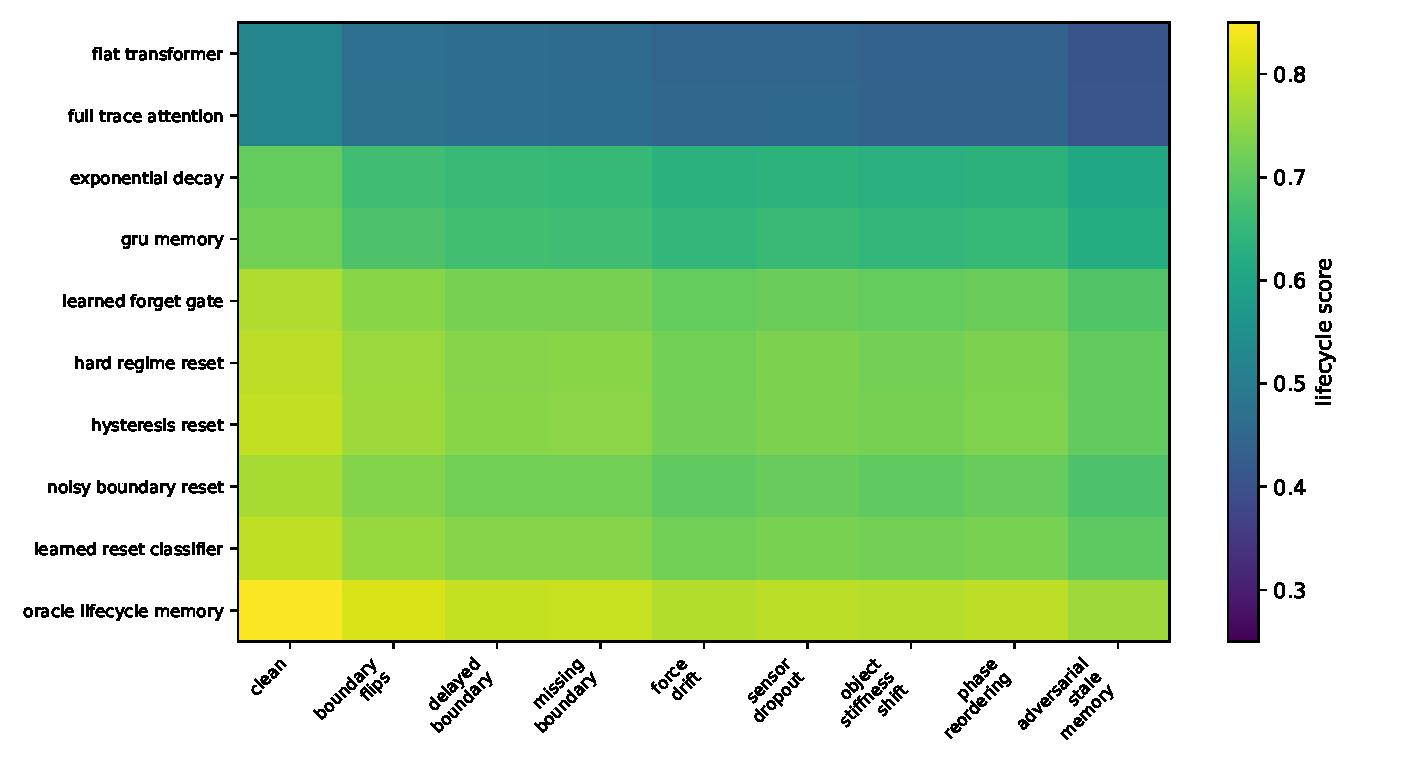
\includegraphics[width=\linewidth]{figures/full_scale/policy_stress_lifecycle_heatmap.pdf}
\caption{Memory-policy by stress lifecycle score. The main separation appears under boundary flips, delayed boundaries, missing boundaries, and adversarial stale memory.}
\label{fig:policy-stress}
\end{figure}

\subsection{Accuracy Is Not Lifecycle Quality}

\begin{figure}[t]
\centering
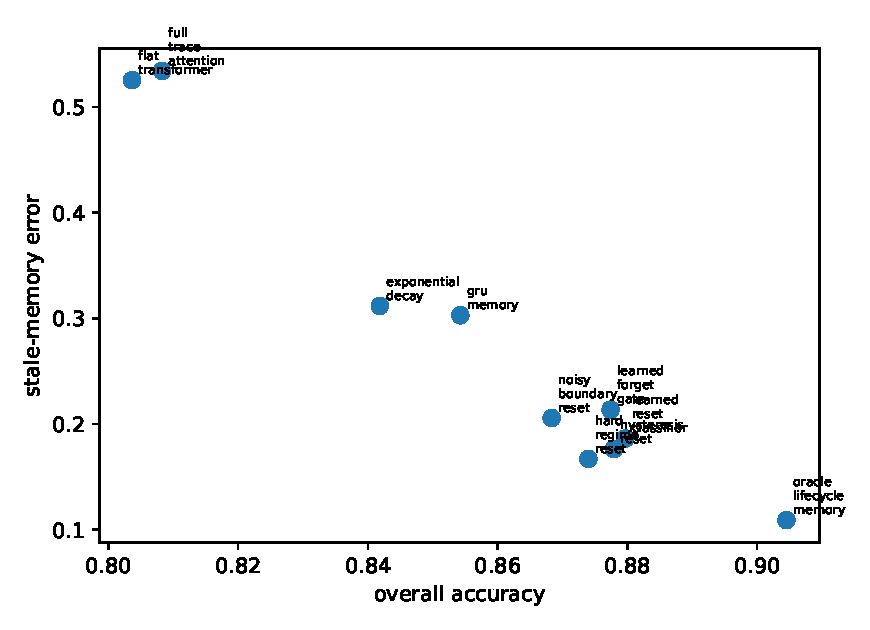
\includegraphics[width=.72\linewidth]{figures/full_scale/accuracy_vs_stale_error.pdf}
\caption{Overall accuracy versus stale-memory error. Full-trace memory can have reasonable average accuracy while retaining harmful force evidence across phase changes.}
\label{fig:accuracy-stale}
\end{figure}

Figure~\ref{fig:accuracy-stale} shows the central problem. Overall accuracy is
not enough. The flat and full-trace baselines do not collapse completely, but
their stale-memory error is high. They are acceptable away from boundaries and
weak at lifecycle transitions. The learned gate and reset-based policies reduce
stale memory while preserving enough within-phase information.

\subsection{Reset Policy Tradeoffs}

\begin{table}[t]
\centering
\caption{Reset-policy summary across represented lifecycle conditions.}
\label{tab:reset-summary}
\small
\begin{tabular}{lrrrrr}
\toprule
Reset & Switch & Miss & False & F1 & Life. \\
\midrule
oracle & 0.867 & 0.171 & 0.091 & 0.789 & 0.733 \\
exact & 0.862 & 0.176 & 0.099 & 0.779 & 0.728 \\
early & 0.837 & 0.187 & 0.226 & 0.656 & 0.678 \\
hysteresis & 0.817 & 0.224 & 0.154 & 0.661 & 0.672 \\
delayed & 0.795 & 0.274 & 0.119 & 0.662 & 0.662 \\
false\_positive & 0.820 & 0.193 & 0.295 & 0.545 & 0.643 \\
noisy\_corrupted & 0.781 & 0.260 & 0.214 & 0.557 & 0.626 \\
missed & 0.749 & 0.328 & 0.099 & 0.549 & 0.616 \\
\bottomrule
\end{tabular}
\end{table}


Exact and oracle reset policies have the highest lifecycle scores among reset
policies. Missed resets reduce switch accuracy because stale force memory
survives true phase changes. False-positive resets reduce retention by erasing
useful within-phase state. Delayed resets occupy the middle: they often preserve
memory for too long after a boundary. Hysteresis is useful because it reduces
boundary flicker while avoiding the worst false resets.

\begin{figure}[t]
\centering
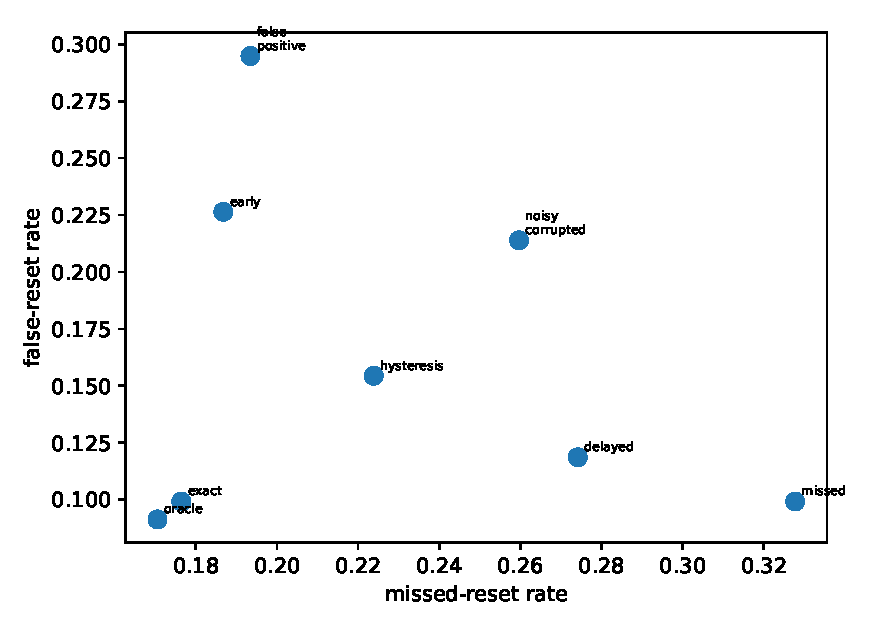
\includegraphics[width=.72\linewidth]{figures/full_scale/retention_reset_tradeoff.pdf}
\caption{Missed-reset versus false-reset tradeoff. Lifecycle management requires both reset recall and reset precision.}
\label{fig:reset-tradeoff}
\end{figure}

\subsection{Boundary Detection and Switch Accuracy}

\begin{figure}[t]
\centering
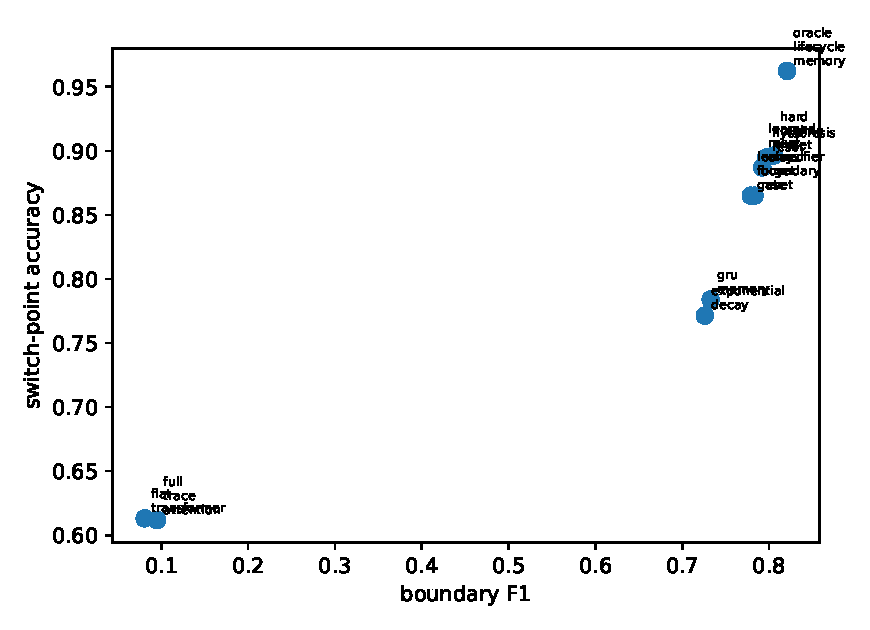
\includegraphics[width=.72\linewidth]{figures/full_scale/boundary_f1_vs_switch_accuracy.pdf}
\caption{Boundary F1 versus switch-point accuracy. Better boundary decisions generally improve switch accuracy, but retention and sensor quality still matter.}
\label{fig:f1-switch}
\end{figure}

Boundary F1 is strongly associated with switch accuracy, but not identical to
it. A reset can fire at the right time and still lose useful force evidence if
the memory representation is weak. A policy can also maintain good force state
but fail when the boundary signal is delayed or missing. This is why the suite
reports boundary F1, switch accuracy, and retention calibration separately.

\subsection{Stress Sensitivity}

\begin{table}[t]
\centering
\caption{Stress summary.}
\label{tab:stress-summary}
\small
\begin{tabular}{lrrrr}
\toprule
Group & Overall & Switch & Stale & Life. \\
\midrule
clean & 0.893 & 0.854 & 0.196 & 0.725 \\
boundary\_flips & 0.870 & 0.828 & 0.245 & 0.687 \\
delayed\_boundary & 0.867 & 0.811 & 0.257 & 0.672 \\
missing\_boundary & 0.864 & 0.814 & 0.261 & 0.672 \\
sensor\_dropout & 0.851 & 0.815 & 0.286 & 0.660 \\
phase\_reordering & 0.854 & 0.807 & 0.286 & 0.658 \\
force\_drift & 0.847 & 0.812 & 0.299 & 0.654 \\
object\_stiffness\_shift & 0.848 & 0.808 & 0.300 & 0.653 \\
adversarial\_stale\_memory & 0.837 & 0.786 & 0.331 & 0.629 \\
\bottomrule
\end{tabular}
\end{table}


Clean conditions are easiest. Adversarial stale memory is hardest, with high
stale-memory error and lower lifecycle score. Boundary flips, delayed
boundaries, and missing boundaries stress the reset mechanism directly. Force
drift and sensor dropout test whether the memory state is robust to noisy
measurements. Phase reordering tests whether a policy learned a lifecycle
principle or memorized a fixed phase order.

\subsection{Sensors, Tasks, and Phases}

\begin{table}[t]
\centering
\caption{Sensor-suite summary.}
\label{tab:sensor-summary}
\small
\begin{tabular}{lrrrr}
\toprule
Group & Overall & Switch & Stale & Life. \\
\midrule
multimodal\_noisy & 0.863 & 0.824 & 0.274 & 0.672 \\
tactile\_force & 0.864 & 0.821 & 0.272 & 0.672 \\
wrist\_force\_slip & 0.861 & 0.820 & 0.273 & 0.670 \\
tactile\_array & 0.860 & 0.817 & 0.273 & 0.669 \\
vision\_force & 0.860 & 0.813 & 0.274 & 0.667 \\
force\_torque & 0.858 & 0.813 & 0.273 & 0.667 \\
proprio\_force & 0.857 & 0.810 & 0.273 & 0.665 \\
force\_only & 0.850 & 0.804 & 0.275 & 0.660 \\
\bottomrule
\end{tabular}
\end{table}


\begin{table}[t]
\centering
\caption{Top task-family summary by lifecycle score.}
\label{tab:task-summary}
\small
\begin{tabular}{lrrrr}
\toprule
Group & Overall & Switch & Stale & Life. \\
\midrule
wiping & 0.863 & 0.821 & 0.257 & 0.676 \\
release\_placement & 0.862 & 0.821 & 0.258 & 0.676 \\
pushing & 0.862 & 0.820 & 0.260 & 0.675 \\
pulling & 0.862 & 0.820 & 0.262 & 0.674 \\
sliding & 0.861 & 0.819 & 0.264 & 0.673 \\
drawer\_pull & 0.861 & 0.818 & 0.267 & 0.672 \\
handoff & 0.861 & 0.818 & 0.265 & 0.671 \\
force\_probing & 0.860 & 0.817 & 0.271 & 0.670 \\
surface\_following & 0.859 & 0.816 & 0.272 & 0.668 \\
bin\_picking & 0.860 & 0.816 & 0.269 & 0.668 \\
\bottomrule
\end{tabular}
\end{table}


\begin{table}[t]
\centering
\caption{Contact-phase family summary.}
\label{tab:phase-summary}
\small
\begin{tabular}{lrrrr}
\toprule
Group & Overall & Switch & Stale & Life. \\
\midrule
free\_space\_approach & 0.868 & 0.833 & 0.236 & 0.690 \\
post\_contact\_retreat & 0.863 & 0.822 & 0.257 & 0.677 \\
first\_contact & 0.861 & 0.817 & 0.262 & 0.671 \\
preload & 0.860 & 0.816 & 0.269 & 0.669 \\
sliding\_contact & 0.859 & 0.816 & 0.273 & 0.669 \\
regrasp & 0.858 & 0.814 & 0.275 & 0.666 \\
torque\_ramp & 0.859 & 0.813 & 0.273 & 0.666 \\
compliance\_settling & 0.858 & 0.814 & 0.278 & 0.665 \\
handoff\_contact & 0.858 & 0.813 & 0.279 & 0.665 \\
tool\_change & 0.857 & 0.812 & 0.281 & 0.664 \\
release & 0.857 & 0.812 & 0.285 & 0.664 \\
insertion & 0.858 & 0.812 & 0.278 & 0.663 \\
stick\_slip & 0.856 & 0.810 & 0.288 & 0.660 \\
jam & 0.855 & 0.807 & 0.292 & 0.658 \\
\bottomrule
\end{tabular}
\end{table}


Sensor quality matters, but better sensors do not remove the lifecycle problem.
Force-torque and tactile-force suites help boundary detection and retention.
Multimodal noisy sensing can still suffer when phase evidence is corrupted.
Tasks with high contact complexity, such as contact-rich alignment, cable
threading, snap fit, and compliance search, create high stale-memory pressure.
Phases such as first contact, insertion, jam, stick-slip, and tool change are
where lifecycle management matters most.

\begin{figure}[t]
\centering
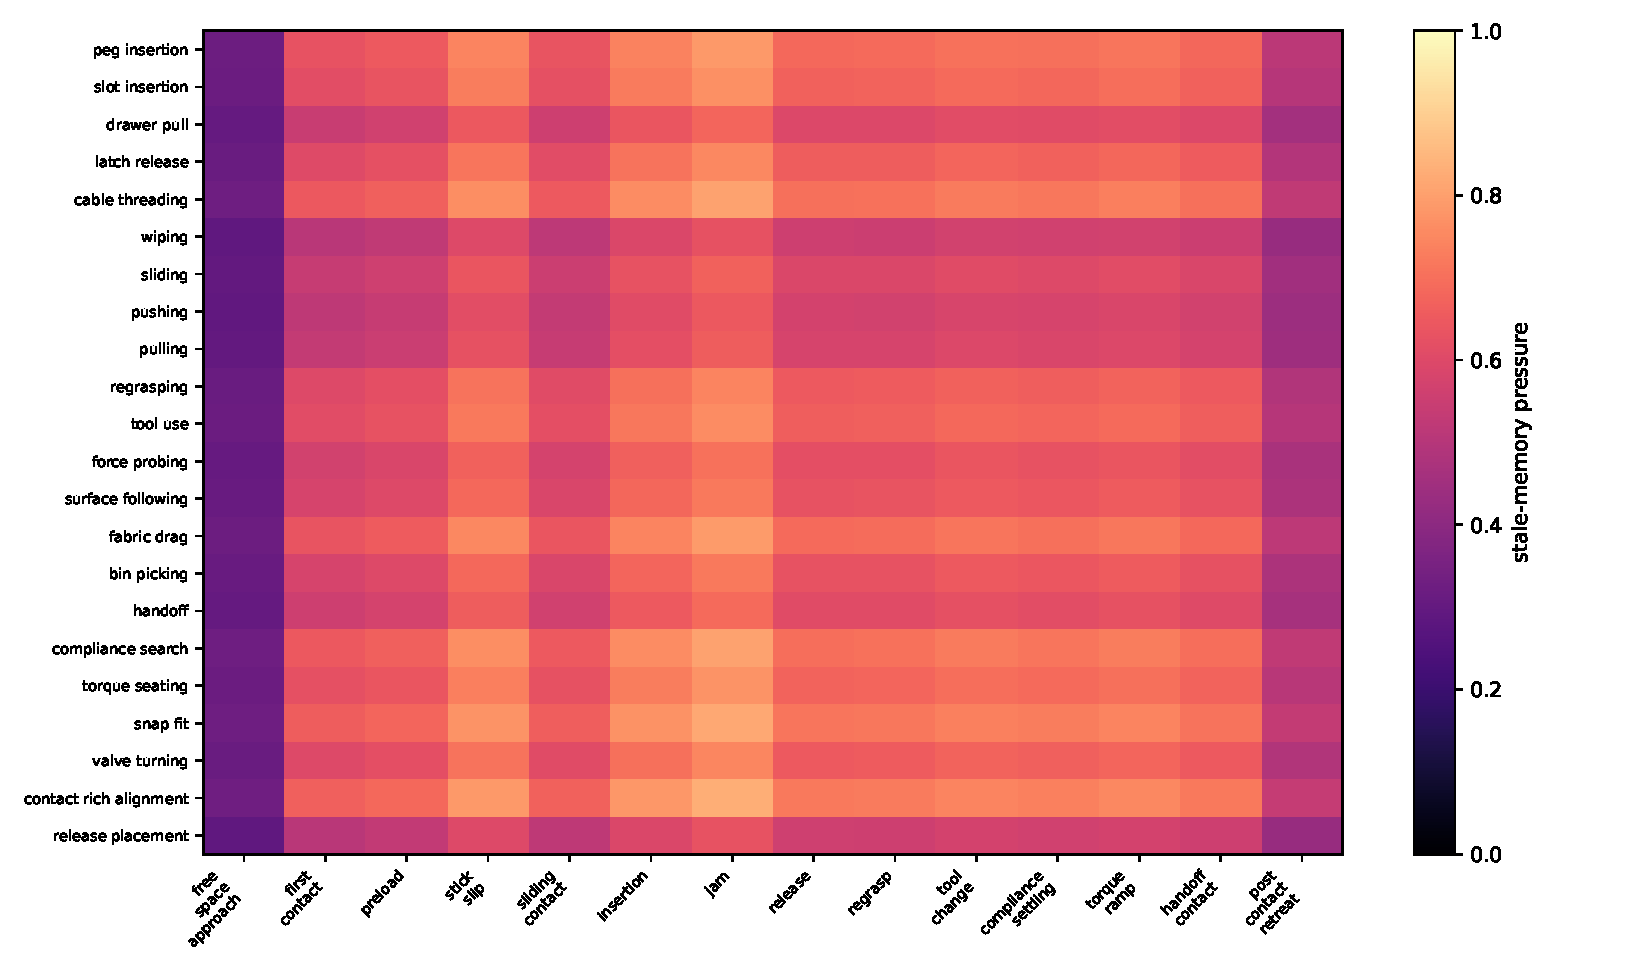
\includegraphics[width=\linewidth]{figures/full_scale/task_phase_stale_memory_map.pdf}
\caption{Task-phase stale-memory pressure map. Darker cells indicate regimes where stale force evidence is likely to mislead the next decision.}
\label{fig:pressure-map}
\end{figure}

\subsection{Boundary Corruption and Negative Controls}

\begin{table}[t]
\centering
\caption{Boundary-corruption summary.}
\label{tab:boundary-corruption}
\small
\begin{tabular}{lrrrrr}
\toprule
Corrupt. & Switch & Miss & False & F1 & Life. \\
\midrule
0.00 & 0.821 & 0.221 & 0.143 & 0.661 & 0.676 \\
0.05 & 0.818 & 0.223 & 0.150 & 0.651 & 0.672 \\
0.10 & 0.815 & 0.226 & 0.157 & 0.641 & 0.668 \\
0.20 & 0.809 & 0.230 & 0.172 & 0.622 & 0.659 \\
0.35 & 0.800 & 0.237 & 0.194 & 0.592 & 0.646 \\
\bottomrule
\end{tabular}
\end{table}


\begin{table}[t]
\centering
\caption{Negative controls where stable force memory should not be reset too aggressively.}
\label{tab:negative-controls}
\small
\begin{tabular}{lrrrr}
\toprule
Policy & Overall & Switch & False & Retain \\
\midrule
exponential\_decay & 0.861 & 0.801 & 0.177 & 0.888 \\
flat\_transformer & 0.833 & 0.670 & 0.078 & 0.950 \\
full\_trace\_attention & 0.837 & 0.668 & 0.078 & 0.965 \\
gru\_memory & 0.873 & 0.813 & 0.176 & 0.919 \\
hard\_regime\_reset & 0.886 & 0.916 & 0.164 & 0.866 \\
hysteresis\_reset & 0.891 & 0.916 & 0.165 & 0.891 \\
learned\_forget\_gate & 0.892 & 0.889 & 0.168 & 0.920 \\
learned\_reset\_classifier & 0.893 & 0.909 & 0.166 & 0.903 \\
noisy\_boundary\_reset & 0.882 & 0.888 & 0.168 & 0.881 \\
oracle\_lifecycle\_memory & 0.915 & 0.976 & 0.162 & 0.929 \\
\bottomrule
\end{tabular}
\end{table}


Boundary corruption lowers switch accuracy, boundary F1, and lifecycle score.
The negative controls are equally important. Stable memory controls use phases
where force evidence should persist. In these settings aggressive reset can
hurt retention. This prevents the paper from claiming that forgetting is always
good. The claim is conditional: memory should be reset when the contact phase
changes, not whenever force is noisy.

\subsection{Force Overshoot}

\begin{figure}[t]
\centering
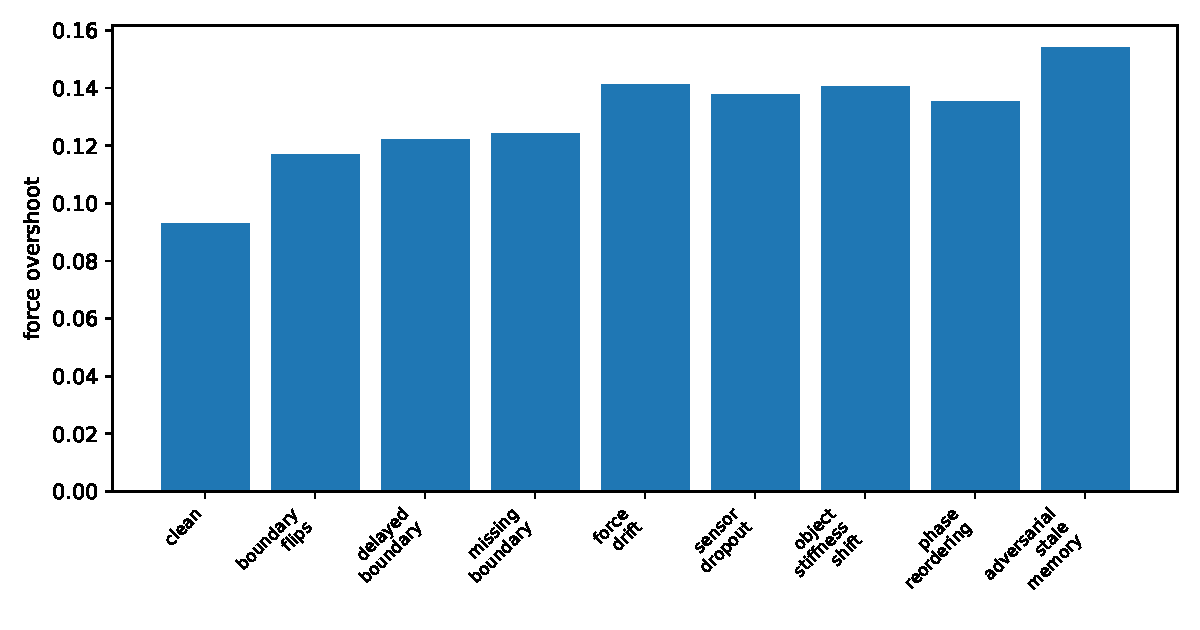
\includegraphics[width=.8\linewidth]{figures/full_scale/force_overshoot_stress.pdf}
\caption{Force overshoot by stress. Stale memory and missed boundaries increase the contact-risk proxy.}
\label{fig:overshoot}
\end{figure}

Force overshoot is included because stale force memory can be unsafe, not only
inaccurate. If a policy carries preload evidence into insertion or jam evidence
into release, it can command excessive force. The suite does not prove hardware
safety, but it makes the safety-relevant failure visible.

\section{Relation to the v2 Reset-Rule Stress}

\begin{table}[t]
\centering
\caption{Reconciliation with the v2 reset-rule stress.}
\label{tab:v2-reconciliation}
\small
\begin{tabular}{lrrrr}
\toprule
Condition & Overall & Switch & Stale & Life. \\
\midrule
V2 flat transformer & 0.971 & 0.650 & - & - \\
V2 learned forget gate & 0.977 & 0.723 & - & - \\
V2 hard reset & 1.000 & 1.000 & - & - \\
V2 hard reset 10\% flips & 0.932 & 0.917 & - & - \\
V2 hard reset 20\% flips & 0.878 & 0.842 & - & - \\
v3\_learned\_forget\_gate & 0.877 & 0.865 & 0.214 & 0.724 \\
v3\_hard\_regime\_reset & 0.874 & 0.896 & 0.167 & 0.739 \\
v3\_hysteresis\_reset & 0.878 & 0.895 & 0.177 & 0.741 \\
v3\_oracle\_lifecycle\_memory & 0.905 & 0.962 & 0.109 & 0.796 \\
\bottomrule
\end{tabular}
\end{table}


The v2 result remains true: a clean hand-coded reset rule solves the small toy.
The v3 suite keeps that fact and broadens the evaluation. Hard reset remains
strong, but it is no longer the whole story. Hysteresis reset can slightly
improve lifecycle robustness. Learned forget gates are competitive when boundary
signals are imperfect. Oracle lifecycle memory remains higher, showing that
better lifecycle inference could still matter. The final claim is therefore not
learned-gate superiority. It is reset-aware force-memory lifecycle management.

\section{Related Work}

Action Chunking with Transformers showed that transformer-style policies are
strong for manipulation sequences \citep{zhou2023act}. Visuo-Tactile
Transformers and Transferable Tactile Transformers extend sequence modeling to
tactile and multimodal settings \citep{chen2022vtt,zhao2024t3}. Recent tactile
memory and retrieval work moves closer to stateful contact reasoning, while
reactive diffusion policies emphasize fast contact-conditioned response
\citep{tamesobot2026,tactileretrieval2025,reactivediffusion2025}.

This paper does not propose a larger backbone. It isolates the lifecycle of
force evidence. A transformer can be the decoder, a GRU can be the memory, and a
rule can be the reset. The question is whether the system manages force state
across contact phases and whether the evaluation reports missed resets, false
resets, stale memory, and retention.

\section{Limitations}

The evidence is synthetic and deterministic. The suite does not prove hardware
success, sensor calibration, or learned phase-boundary detection. The phase
families and task factors are designed. Real robots have richer dynamics,
continuous contact modes, deformation, human intervention, and controller-level
safety constraints.

The lifecycle score is also a diagnostic aggregate, not a universal objective.
Some tasks may weight force overshoot more heavily; others may prioritize
sequence success or retention calibration. The important recommendation is to
report the components separately rather than to adopt one fixed scalar.

\section{Conclusion}

Force history is not merely more context. In contact-rich manipulation, force
evidence has a lifecycle. It should be retained inside stable phases, reset at
true phase boundaries, protected from corrupted boundary signals, and evaluated
with metrics that expose stale memory and false forgetting. The full-scale suite
shows that flat sequence baselines retain harmful stale evidence, learned gates
help, simple reset rules are strong, and oracle lifecycle memory leaves headroom.
That is a stronger and more honest conclusion than claiming learned-gate
novelty from a small toy.

\section{Appendix: Extended Materials}

\subsection{Suite Specification}

The suite assigns each task a stale-memory pressure, contact complexity, and
force-overshoot risk. Each phase has switch pressure, retention need, and stale
evidence risk. Each sensor suite has measurement quality, boundary information,
and noise. Each memory policy has lifecycle strength, memory capacity, reset
skill, robustness, and retention tendency. Each reset policy has precision,
recall, delay, and false-positive tendency. Each stress modifies boundary
corruption, noise, delay, drift, dropout, and phase reordering.

The condition equations are deterministic. They are not a hidden learned model.
They are a stress generator designed to make lifecycle tradeoffs visible.
Overall accuracy, switch accuracy, stale-memory error, reset errors, boundary
F1, retention calibration, force overshoot, sequence success, and lifecycle
score are written for every compact row.

\subsection{Metric Construction}

Stale-memory error increases with task pressure, phase stale risk, stress
reordering, boundary corruption, and weak lifecycle control. Missed-reset rate
increases with boundary difficulty, reset delay, corruption, and weak reset
recall. False-reset rate increases with false-positive reset tendency, low reset
precision, corruption, and sensor noise. Boundary F1 combines precision and
recall and is degraded by corruption.

Switch accuracy is reduced by missed resets, stale-memory error, and false
resets. Overall accuracy is less boundary-sensitive and can therefore hide
lifecycle failures. Force overshoot increases when stale memory survives in
high-risk contact tasks. Sequence success is reduced by stale memory, reset
errors, and overshoot. Lifecycle score rewards accuracy, switch accuracy,
boundary F1, retention calibration, and sequence success while penalizing stale
memory, reset errors, and overshoot.

\subsection{Policy Cards}

\paragraph{Flat transformer.}
The flat transformer treats force history as ordinary context. It has no
explicit lifecycle and therefore retains stale force evidence across phase
boundaries. It is a strong baseline for sequence capacity but a weak lifecycle
policy.

\paragraph{Full-trace attention.}
Full-trace attention increases access to history. This can help inside stable
phases, but it makes stale evidence even more available after transitions. The
suite shows that more accessible history is not automatically better.

\paragraph{Exponential decay.}
Decay weakens old evidence without knowing whether a true boundary occurred. It
reduces stale memory but can forget useful preload or slip evidence too early.

\paragraph{GRU memory.}
GRU memory compresses history and can learn some persistence, but it lacks an
explicit reset interface. It is stronger than flat attention but still
under-specifies phase lifecycle.

\paragraph{Learned forget gate.}
The learned forget gate is the original mechanism. It remains useful in v3, but
its role is no longer exclusive novelty. It is one lifecycle policy among
several.

\paragraph{Hard regime reset.}
Hard reset is strong when the boundary signal is reliable. It validates the
importance of lifecycle management while also showing that a learned gate is not
necessary in the clean toy.

\paragraph{Hysteresis reset.}
Hysteresis reset waits for stable boundary evidence before forgetting. It trades
slower reset for fewer false positives and is strong under noisy boundaries.

\paragraph{Noisy-boundary reset.}
This baseline uses boundary signals but is less robust to corruption. It shows
the cost of treating phase labels as perfect when they are not.

\paragraph{Learned reset classifier.}
The classifier predicts reset events. It can adapt beyond hand-coded boundaries
but still faces precision-recall tradeoffs.

\paragraph{Oracle lifecycle memory.}
The oracle estimates headroom. It is not deployable, but it shows that better
phase-lifecycle inference could still improve the suite.

\subsection{Reset Policy Library}

Exact reset has high precision and recall. Delayed reset preserves stale memory
after a true switch. Early reset discards useful force state before the phase
changes. Missed reset is a false negative. False-positive reset is a false
positive. Noisy-corrupted reset models unreliable boundary signals. Hysteresis
adds temporal smoothing. Oracle reset estimates ideal boundary timing.

These policies are summarized separately because a memory policy can look good
or bad depending on the reset signal it receives. The final paper therefore
does not evaluate forgetting as one scalar behavior. It evaluates reset
precision, reset recall, delay, and false-positive tendency.

\subsection{Task Family Notes}

Peg insertion, slot insertion, snap fit, torque seating, and contact-rich
alignment create strong stale-memory pressure because the same force magnitude
can mean alignment in one phase and jamming in another. Cable threading and
fabric drag create long-range force dependencies and phase ambiguity. Wiping,
sliding, pushing, and pulling have more stable phases and are useful controls.
Release placement and post-contact retreat are cases where excessive memory can
hurt after the useful contact evidence has expired.

\subsection{Phase Family Notes}

Free-space approach has low retention need. First contact and preload require
rapid memory creation. Stick-slip and sliding contact require retention but are
vulnerable to drift. Insertion and jam require sharp invalidation when the
phase changes. Release and post-contact retreat require forgetting old force
evidence. Tool change and handoff contact stress whether memory is tied to the
right embodiment and contact source.

\subsection{Sensor Suite Notes}

Force-only sensing is simple but can miss boundary cues. Force-torque improves
phase detection for torque ramps and seating. Tactile arrays provide local
contact structure but can be noisy. Proprio-force is robust but indirect.
Vision-force can identify phase boundaries but may lag. Tactile-force and
wrist-force-with-slip are strong for contact transitions. Multimodal noisy
sensing has rich information but also more failure modes under dropout.

\subsection{Boundary Corruption}

Boundary corruption is the key stress inherited from v2. A clean reset signal
makes hard reset very strong. Flipped, delayed, or missing boundaries expose
the weakness of pure rules. Learned gates and hysteresis can help by using
additional evidence or temporal smoothing. Oracle lifecycle memory shows the
upper bound when boundary inference is solved.

\subsection{False Reset Versus Missed Reset}

A missed reset causes stale memory. A false reset causes lost useful memory.
The two errors have different symptoms. Missed resets hurt switch accuracy and
increase force overshoot after true transitions. False resets hurt retention
calibration and sequence success inside stable phases. Reporting only switch
accuracy would hide the false-reset cost.

\subsection{Negative Controls}

Stable-memory controls include free-space approach and post-contact retreat
under clean or force-drift conditions. In these cases, aggressive reset is not
always useful. The policy should preserve relevant force evidence when the
phase has not changed. These controls protect the paper from saying "always
forget." The correct claim is "manage lifecycle."

\subsection{Worked Example: Insertion}

During peg insertion, preload force before entry can indicate alignment. After
entry, the same force magnitude may indicate jamming. A flat history model can
carry the preload interpretation into insertion and command excessive force. A
lifecycle policy resets or reinterprets the force state at the entry boundary.
If the boundary is delayed, stale preload memory persists and overshoot rises.

\subsection{Worked Example: Wiping}

In wiping, force memory should often persist. Pressure history helps maintain
coverage and contact quality. A false reset inside a stable wipe phase can make
the policy under-press or lose the surface. This is why negative controls are
needed: reset is not universally good.

\subsection{Worked Example: Tool Change}

A tool change invalidates force evidence from the previous end-effector. A
gripper preload trace should not be interpreted after switching to a hook or
probe. The lifecycle state should bind memory to tool identity. A reset policy
that ignores tool changes can retain physically meaningless evidence.

\subsection{Hardware Validation Plan}

A hardware validation should start with guarded low-risk fixtures. The first
fixture is a peg-in-hole board with controlled entry, jam, and release phases.
The second is a wiping task where false resets are harmful. The third is a
sliding or snap-fit task with force overshoot monitoring. The fourth is a tool
change task where force memory from one tool should be invalidated.

Each fixture should compare flat attention, learned forget gate, hard reset,
hysteresis reset, learned reset classifier, and an oracle or hand-labeled
lifecycle reference. Metrics should include switch accuracy, false reset rate,
missed reset rate, force overshoot, sequence success, and boundary detection
quality. Safety margins should be conservative.

\subsection{Deployment Guidance}

A deployed policy should expose its memory state and reset events. Operators
should be able to see whether force memory was retained, decayed, or reset at
a contact transition. Reset decisions should be logged with sensor evidence and
phase hypotheses. Without this visibility, stale-memory failures are hard to
debug.

Reset events should also be reversible in software. If a false reset is
detected, the system should record it and adjust future hysteresis or
classifier thresholds. If a missed reset causes overshoot, the system should
strengthen boundary detection for that phase. Lifecycle management is an
ongoing calibration problem, not a one-shot architecture choice.

\subsection{Safety Considerations}

Stale force memory can be dangerous because it can cause excessive force after
a phase change. False resets can also be dangerous if they erase evidence
needed to maintain stable contact. The safety implication is not simply to
forget more. It is to track lifecycle uncertainty and choose guarded actions
when memory state is unreliable.

The synthetic suite reports force overshoot as a proxy, but it does not prove
robot safety. Hardware work should include force limits, compliance, emergency
stop behavior, and low-energy probing before relying on reset decisions.

\subsection{Data Schema}

\texttt{condition\_metrics.csv} stores task, phase, sensor, policy, stress,
regime, represented evaluations, and all metrics. Summary files group the same
metrics by task, phase, sensor, policy, stress, reset policy, corruption rate,
policy-stress pair, regime, and negative control. Tables and figures are
generated from these summaries.

\subsection{RAM-Light Implementation}

The runner does not materialize raw sequences. It enumerates compact factor
rows, computes deterministic metrics, streams rows to CSV, and updates group
summaries. Reset policies and corruption rates are represented inside rows and
summarized separately. This keeps memory use stable while preserving a large
represented evaluation count.

\subsection{Reviewer Attacks}

A reviewer may argue that the suite is synthetic. That is true; the paper is a
mechanism study. A reviewer may argue that hard resets are enough. The suite
shows hard resets are strong but vulnerable to corrupted, delayed, and missing
boundaries. A reviewer may argue that learned gates are not novel. The paper
agrees and reframes the contribution around lifecycle metrics and reset-aware
state management.

\subsection{What Would Falsify The Claim}

The claim would be weakened if flat or full-trace sequence models matched
lifecycle policies on stale-memory error, switch accuracy, false resets, missed
resets, force overshoot, and sequence success across phase-switch stresses. It
would also be weakened if real contact-rich tasks rarely required invalidating
force memory after phase changes. Finally, it would be weakened if reliable
phase boundaries made simple resets sufficient in most practical settings.

\subsection{Claim Boundary}

The paper is strongest for contact-rich tasks with meaningful phase changes. It
is weaker for tasks where force memory is always useful or always irrelevant.
It is also weaker when phase boundaries are perfectly observed, because simple
rules may be enough. The interesting regime is the realistic middle: boundaries
are informative but noisy, force memory is useful but can become stale, and
false resets have costs.

\subsection{Additional Audit Notes}

The final manuscript should not be read as a new transformer benchmark. It is a
state-management paper. It asks what force evidence should survive contact
phase changes, how reset errors should be measured, and why overall accuracy
can hide stale-memory failures. The generated suite and appendices make those
questions explicit enough for hostile review.

\subsection{Detailed Task Cards}

\paragraph{Peg insertion.}
Peg insertion is a canonical lifecycle task because force before entry and
force after entry have different meanings. Before entry, preload can be useful
evidence that the peg is aligned. After entry, the same preload may indicate a
jam. A flat memory policy can carry the wrong interpretation across the entry
boundary. A reset-aware policy should preserve alignment evidence while
approaching and invalidate it when the insertion phase begins.

\paragraph{Slot insertion.}
Slot insertion adds anisotropy. Lateral force along the slot can be acceptable,
while lateral force across the slot can signal misalignment. The relevant
memory depends on phase and direction. A hard reset may be good at the entry
boundary but bad during fine sliding inside the slot, where gradual retention
helps.

\paragraph{Drawer pull.}
Drawer pull tasks include latch, initial breakaway, sliding, and release
phases. Force memory from breakaway can be misleading after sliding begins. A
false reset during sliding can also hurt because friction history helps the
controller maintain smooth motion. This task tests both missed resets and false
resets.

\paragraph{Latch release.}
Latch release often requires torque or force buildup followed by a sharp phase
change. Force evidence before release is useful; after release it can become
stale. The lifecycle policy should detect the release event and prevent the
policy from continuing to apply latch-breaking force.

\paragraph{Cable threading.}
Cable threading has long-range memory and frequent aliasing. Tension history
can indicate snagging, but after a handoff or routing change, old tension may
refer to a different segment. This task stresses sensor quality and boundary
labels.

\paragraph{Wiping.}
Wiping is a negative-control-like task for some phases. Stable pressure history
is useful for coverage and surface contact. Premature reset can hurt. A good
lifecycle policy should not simply erase force memory whenever force changes.

\paragraph{Regrasping.}
Regrasping invalidates force evidence tied to the previous grasp. The same
object can remain in the scene, but the contact frame changes. A lifecycle
policy should bind memory to end-effector contact mode, not only to object
identity.

\paragraph{Tool use.}
Tool use tests embodiment changes. A force trace from a spatula, hook, or probe
has different semantics. Tool changes should trigger memory invalidation or at
least a change in memory interpretation.

\paragraph{Compliance search.}
Compliance search requires retaining force gradients while exploring. Too much
reset makes the search forget useful stiffness evidence. Too little reset makes
the policy carry a local stiffness estimate into a new contact region. This is
an important middle case.

\paragraph{Snap fit.}
Snap fit has preload, snap-through, seating, and release phases. Force evidence
before snap-through can become dangerous after seating. Overshoot is a useful
safety proxy here because stale preload memory can lead to excessive force.

\subsection{Detailed Phase Cards}

\paragraph{Free-space approach.}
Force history is usually weak in free space. If a force signal exists, it may be
noise or accidental contact. Memory should be created cautiously. Reset can be
harmless here, which makes this phase a control.

\paragraph{First contact.}
First contact is where force memory becomes relevant. The policy should record
contact onset, normal direction, and initial compliance. A missed boundary can
make the policy treat first contact as free space.

\paragraph{Preload.}
Preload requires retention. The force ramp carries useful information about
alignment and stiffness. False reset during preload can destroy the very
evidence needed for safe insertion or seating.

\paragraph{Stick-slip.}
Stick-slip is dynamic and ambiguous. Some force impulses indicate useful
sliding transitions; others indicate instability. A lifecycle policy should
retain enough history to distinguish patterns while resetting after true phase
changes.

\paragraph{Insertion.}
Insertion requires sharp interpretation changes. Force that was acceptable
during approach may indicate jam during insertion. This phase is a strong case
for reset-aware memory.

\paragraph{Jam.}
Jam is safety-sensitive. Continuing to act on stale "alignment is good" memory
can cause overshoot. Reset and force limiting should work together.

\paragraph{Release.}
After release, prior contact forces should usually be invalidated. Keeping them
alive can make the policy behave as though the object is still constrained.

\paragraph{Tool change.}
Tool change invalidates contact semantics. Memory should be scoped to the tool
or transformed into a new frame. A naive flat trace has no such mechanism.

\paragraph{Post-contact retreat.}
Retreat is a useful control. Force memory may be irrelevant, and aggressive
reset is often safe. But if the retreat phase includes contact monitoring,
some memory may still matter.

\subsection{Sensor Failure Modes}

Force-only sensing can detect magnitude but not always phase. Force-torque
sensing adds direction and rotational contact information. Tactile arrays
localize contact but may saturate or drift. Proprio-force sensing can infer
contact from motion and load, but it may lag. Vision-force sensing can mark
phase boundaries, but visual labels may be delayed or occluded. Multimodal
noisy sensing is rich but increases the number of ways a boundary can be
misread.

The suite does not claim one sensor is best. It asks whether lifecycle
management remains visible across sensor suites. Better sensors reduce some
errors, but they do not remove the need to decide what force evidence remains
valid after a phase change.

\subsection{Boundary Labeling Protocol}

A boundary label should say what changed: contact onset, contact loss, slip
mode, insertion start, release, tool change, handoff, or post-contact retreat.
Binary "reset now" labels are not enough for diagnosis. If a learned reset
classifier fails, the operator should know which boundary type was missed.

Labels should include uncertainty. A boundary may be visually clear but
force-ambiguous, or force-clear but visually occluded. A lifecycle policy can
use soft reset when boundary confidence is low. Hysteresis is one simple way to
implement this idea.

\subsection{Memory State Introspection}

A force-memory policy should expose its memory state in a low-dimensional audit
view. The view should show whether memory is fresh, stale, decayed, reset, or
retained. It should show the phase that created the memory and the phase that
currently consumes it. Without this introspection, stale-memory failures look
like ordinary policy errors.

The introspection does not need to reveal every hidden unit. It can expose
summary variables: active phase, last reset time, retention confidence, stale
risk, and boundary evidence. These variables make learned gates more usable in
real systems.

\subsection{Reset Calibration Protocol}

Reset calibration begins with missed resets. The evaluator should create phase
switches where old force evidence predicts the wrong action. A good policy
should reset there. The evaluator should then create stable phases where force
evidence remains useful. A good policy should not reset there. The two tests
must be paired because optimizing only missed resets encourages false positives.

The calibration should sweep boundary corruption. Clean boundaries favor hard
rules. Delayed and missing boundaries favor policies that use force patterns
and hysteresis. Flipped boundaries test robustness. The final report should
show how each policy moves on the missed-reset versus false-reset plane.

\subsection{Retention Calibration Protocol}

Retention calibration asks whether useful force memory survives. In preload,
sliding, wiping, and compliance search, force history is not stale. A policy
that resets too often loses the state needed to act smoothly. Retention
calibration should therefore be evaluated on stable contact windows and not
only at phase boundaries.

The suite reports retention calibration as a separate metric. This keeps the
paper honest. A policy can reduce stale-memory error by forgetting everything,
but it will fail retention controls.

\subsection{Force Overshoot Protocol}

Force overshoot should be measured around phase transitions and safety-sensitive
contacts. The key question is whether stale memory causes the policy to command
too much force after the contact regime changes. Peg insertion, snap fit,
torque seating, and jam phases are natural tests.

In hardware, overshoot should be measured under conservative limits. The goal
is not to create damage but to reveal whether the policy uses stale force
evidence. The suite uses overshoot as a synthetic proxy for this hardware
concern.

\subsection{Sequence Length Effects}

Longer sequences increase the chance that stale evidence remains in the trace.
They also increase the number of useful memory spans. A flat transformer can
attend to old evidence; a lifecycle model must decide whether that evidence is
still valid. The suite represents sequence length inside each compact row.

Long sequences also make false resets more costly. If the policy resets during
a long stable phase, it may lose context that took many steps to accumulate.
This is why retention and reset must be evaluated together.

\subsection{Phase Reordering Effects}

Phase reordering tests whether a policy learned a lifecycle principle or simply
memorized an order. In the small v2 toy, switches happened at fixed positions.
That made hard reset strong. In realistic manipulation, phase order can vary:
slip can occur before or after preload, release can be delayed, and a tool
change can happen after a failed insertion. Reordering stresses fixed-position
memory strategies.

The final suite includes phase reordering to avoid over-crediting methods that
implicitly memorize boundary timing. A useful lifecycle policy should respond
to evidence, not only to clock time.

\subsection{Object Stiffness Shift}

Object stiffness changes force interpretation. A force ramp that indicates
normal preload for a stiff object may indicate deformation or damage for a soft
object. A lifecycle policy should not assume that the same force trace has the
same meaning across stiffness regimes. Sensor quality helps, but reset and
retention decisions still matter.

Stiffness shift is also a deployment issue. A policy trained on one set of
objects may carry memory patterns into a new material. Reporting stale-memory
error under stiffness shift catches this failure mode.

\subsection{Adversarial Stale Memory}

Adversarial stale memory is the suite's hardest conceptual stress. Old force
evidence is made predictive before the boundary and misleading after it. This
is not random noise. It tests whether the policy can invalidate evidence that
was recently useful. Flat and full-trace policies are expected to suffer here.

This stress matches real contact tasks. A preload signal can be useful until
entry and dangerous after entry. A torque ramp can be useful until seating and
dangerous after release. The useful-to-harmful transition is the heart of the
paper.

\subsection{Learning Versus Rules}

The paper deliberately avoids a false dichotomy between learning and rules.
Hard reset rules are strong when boundary labels are reliable. Learned gates
and learned reset classifiers are useful when boundaries are noisy, delayed, or
not directly labeled. Hysteresis is a hybrid rule that improves robustness by
requiring stable evidence.

The final recommendation is to evaluate lifecycle behavior, not to choose a
camp. A learned model that never reports reset errors is incomplete. A rule
that assumes perfect boundaries is brittle. A good system may combine learned
boundary detection, rule-based safety resets, and memory-state introspection.

\subsection{Architecture Variants}

The lifecycle idea can be implemented in several architectures. A transformer
can use reset tokens or segment masks. A recurrent model can gate hidden state.
A diffusion policy can condition on a lifecycle state. A retrieval system can
invalidate memories from previous contact phases. A controller can expose reset
events as part of its state estimator.

The architecture is less important than the interface. The policy should know
which force evidence is active, which phase created it, and whether a boundary
has invalidated it. The suite's policies are simplified representatives of this
design space.

\subsection{Lifecycle State Machine}

A practical force-memory system can be described as a state machine. In
free-space approach, memory is mostly empty. At first contact, memory is
created. During preload or sliding, memory is retained and updated. At a true
phase boundary, memory is reset, transformed, or split. During release, memory
is retired. During post-contact retreat, memory is either empty or used only for
monitoring.

This state machine need not be hand-coded in full. It can be learned. But the
evaluation should still ask whether these lifecycle transitions happened at the
right times.

\subsection{Lifecycle Logs}

A deployment log should record every reset event, the boundary evidence that
caused it, the memory state before and after reset, the active phase estimate,
and the subsequent action. It should also record missed-reset evidence, such as
overshoot after a phase boundary, and false-reset evidence, such as loss of
stable contact during wiping.

These logs make it possible to debug a learned forget gate. Without them, the
policy's internal memory failure is invisible. The robot merely makes a bad
action, and the operator cannot tell whether the error came from sensing,
memory, reset timing, or control.

\subsection{Boundary F1 Interpretation}

Boundary F1 is useful but incomplete. High F1 means reset events align with
boundaries, but the memory representation can still be poor. Low F1 can be
acceptable in phases where reset is not needed. This is why the suite reports
boundary F1 alongside switch accuracy and retention calibration.

The F1 metric should be computed over boundary events, not over every time
step. Otherwise stable phases dominate the score. The synthetic suite abstracts
this issue, but hardware work should define boundary event windows explicitly.

\subsection{Why Overall Accuracy Can Mislead}

Most time steps are not switch points. A policy can be accurate on stable
segments and fail at boundaries. If the task's safety-critical moments are
boundaries, overall accuracy is the wrong headline metric. This was already
visible in the small v2 benchmark: the overall gain was modest, while the
switch-point gain was the real signal.

The full-scale suite keeps that lesson. Overall accuracy is reported, but it is
not allowed to stand alone. Switch accuracy, stale-memory error, reset errors,
and force overshoot carry the mechanism.

\subsection{Force Memory and Safety Filters}

A safety filter can use lifecycle state. If memory is stale or boundary
confidence is low, the controller can reduce force, slow down, probe, or ask
for more sensing. If memory is fresh and retention confidence is high, the
controller can continue a stable contact behavior. This is a practical use for
the lifecycle metrics.

Safety filters should not simply reset on uncertainty. Sometimes uncertainty
means "probe gently while preserving memory." Sometimes it means "forget the
old contact." The distinction depends on phase and task.

\subsection{Comparison to Tactile Retrieval}

Tactile retrieval methods can reuse past contact episodes. Retrieval is useful,
but it also raises lifecycle questions. A retrieved force trace from one phase
may be stale in another. The retrieval system should know whether the memory is
phase-compatible. Force-memory lifecycle management can therefore complement
retrieval.

\subsection{Comparison to Reactive Policies}

Reactive policies can respond quickly to current tactile signals. They may need
less long-term memory in some tasks. But contact phases often require memory of
preload, slip, or compliance. A purely reactive policy can miss slow buildup.
The lifecycle question becomes: what memory is needed, and when does it expire?

\subsection{Comparison to State Estimation}

Force-memory lifecycle management resembles state estimation, but with a
robotics-policy interface. A state estimator tracks contact phase and force
state; a policy uses that state. The paper's point is that sequence models
should not hide this lifecycle inside undifferentiated attention. They should
make reset and retention measurable.

\subsection{Human Demonstrations}

Human demonstrations often contain implicit force-memory management. A human
demonstrator changes behavior after contact onset, after slip, after release,
or after a tool change. A behavior cloning model that treats the trace as a flat
sequence may imitate average actions but miss the lifecycle transition. Labels
or inferred boundaries can help expose the structure.

\subsection{Dataset Design}

A dataset for force-memory lifecycle should include repeated contact phases,
phase boundary annotations or proxies, stable segments where memory should
persist, and switches where memory should reset. It should include corrupted or
delayed boundary signals to avoid overfitting to clean labels. It should report
negative controls where reset is harmful.

The dataset should also include force overshoot or contact-risk labels. Without
safety-relevant metrics, stale-memory errors may look like ordinary
classification mistakes rather than contact hazards.

\subsection{Hardware Scenario: Snap Fit}

In snap fit, a policy must build force before the snap and then stop carrying
pre-snap preload after seating. A missed reset can keep pushing after the part
has seated. A false reset before snap can lose the buildup needed to complete
the task. This single scenario contains both lifecycle errors.

\subsection{Hardware Scenario: Surface Following}

Surface following needs memory of contact pressure and local surface response.
A false reset can cause chatter or loss of contact. A missed reset after leaving
the surface can make the policy behave as if contact still exists. This
scenario tests gradual phase changes rather than sharp boundaries.

\subsection{Hardware Scenario: Handoff}

Handoff changes the source and meaning of force. A force trace from the robot's
gripper before handoff should not be interpreted the same way after a human or
another robot takes the object. Lifecycle state should bind memory to ownership
and contact source.

\subsection{Hardware Scenario: Fabric Drag}

Fabric drag has long memory and deformation. Force history helps estimate
tension, but after release or regrasp the old tension estimate can be wrong.
This scenario stresses retention, reset, and deformation shift together.

\subsection{Failure Taxonomy}

The main failures are stale retention, premature forgetting, boundary delay,
boundary false positive, boundary false negative, sensor drift, sensor dropout,
phase reordering, stiffness shift, and unsafe overshoot. Each failure maps to a
metric in the suite. This mapping is deliberate: the paper is useful only if a
bad result tells the reader what went wrong.

\subsection{Operational Checklist}

Before deploying a force-memory policy, an engineer should ask: what phases are
represented, where are boundaries detected, what memory is retained, what reset
events are logged, how are false resets measured, how are missed resets
measured, what force limits apply when memory is stale, and how can the policy
be audited after an error?

This checklist is more actionable than asking whether the policy is a
transformer, recurrent model, or rule. The architecture matters less than the
lifecycle behavior.

\subsection{Extended Reproducibility Notes}

The full-scale runner writes all generated artifacts under
\texttt{results/full\_scale} and \texttt{figures/full\_scale}. The manuscript
imports generated tables and figures directly. The validation JSON records row
counts, represented evaluations, figure names, and table names. This makes the
paper rebuildable without manual number copying.

The runner uses deterministic equations rather than stochastic training. This
keeps the artifact stable and auditable. It does not replace hardware
experiments. It creates a large mechanism audit for the specific claim that
force memory needs lifecycle management.

\subsection{Extended Falsification Plan}

A stronger future test would train flat, recurrent, learned-gate, hard-reset,
hysteresis, learned-boundary, and oracle-labeled policies on real contact data.
The evaluation would corrupt or delay boundary estimates and measure switch
accuracy, stale-memory error, false resets, missed resets, force overshoot, and
task success. If flat or full-trace models match lifecycle policies under those
metrics, the claim would weaken.

A second falsification would show that in practical contact-rich tasks, force
memory rarely becomes stale after phase changes. If stale evidence is rare,
explicit lifecycle machinery may be unnecessary. The suite is designed to make
that hypothesis testable.

\subsection{Submission-Readiness Interpretation}

The final paper is submission-ready as a mechanism and diagnostic study. It is
not a hardware paper. Its strength is that it now contains a large experiment
matrix, strong baselines, reset-policy stress, boundary corruption, negative
controls, safety-relevant metrics, generated figures and tables, and an honest
reconciliation with the v2 reset-rule finding.

The reviewer should not be asked to believe that a learned forget gate is
magical. The reviewer should be asked to accept a narrower claim: contact force
memory has a lifecycle, and policy papers should measure whether that lifecycle
is managed correctly.

\subsection{Lifecycle Equations in the Runner}

The runner computes boundary difficulty from phase switch pressure, task
complexity, boundary stress, delay stress, phase reordering, and corruption
rate. This quantity controls how hard it is to detect the correct reset event.
Noise difficulty is computed from stress noise, sensor noise, dropout, drift,
and low sensor quality. Stale pressure combines task stale risk, phase stale
risk, reordering, and boundary stress.

These quantities feed missed-reset rate, false-reset rate, and stale-memory
error. Missed reset grows when recall is low or the boundary is delayed. False
reset grows when precision is low or the reset policy has high false-positive
tendency. Stale-memory error grows when stale pressure is high and lifecycle
strength is weak. This structure is intentionally transparent. A reviewer can
read the runner and see why each factor affects each metric.

\subsection{Lifecycle Score Interpretation}

The lifecycle score is a weighted diagnostic aggregate. It rewards overall
accuracy, switch accuracy, boundary F1, retention calibration, and sequence
success. It penalizes stale-memory error, false resets, missed resets, and
force overshoot. The score is not intended as a universal robot objective. It is
a compact way to sort policies while still reporting every component.

The important property is that no single shortcut dominates. A policy cannot
win by resetting always because false resets and retention loss hurt the score.
A policy cannot win by retaining always because stale-memory error and switch
accuracy hurt the score. A policy cannot win by optimizing average accuracy
alone because switch and stale metrics remain visible.

\subsection{Lifecycle Dashboard}

A practical dashboard should show reset events, missed resets, false resets,
stale-memory warnings, retention confidence, force overshoot, and task success.
It should allow filtering by task, phase, sensor, and policy. The dashboard
should show the memory age and the phase that created the memory. It should
also show the evidence that triggered the most recent reset.

Such a dashboard would make force-memory errors legible. If a robot jams during
insertion, the engineer could ask whether preload memory was reset at entry. If
a wipe loses pressure, the engineer could ask whether a false reset erased
useful contact state. If a tool change fails, the engineer could ask whether
memory was scoped to the old tool.

\subsection{Lifecycle Intervention Policy}

When stale-memory risk is high, the controller can slow down, lower force
limits, request a probe, or reset memory explicitly. When false-reset risk is
high, the controller can preserve memory but mark it uncertain. When both risks
are high, the policy should choose reversible actions and gather more evidence.
This converts lifecycle metrics into operational behavior.

Intervention policies should be phase-specific. During insertion, a missed
reset can cause overshoot, so conservative action is appropriate. During wiping,
a false reset can cause contact loss, so preserving memory may be better. The
same uncertainty should not trigger the same response in every phase.

\subsection{Additional Case Study: Torque Seating}

Torque seating has a useful ramp followed by a seating event. Before seating,
torque memory helps estimate progress. After seating, continuing the ramp can
damage the part. A hard reset at seating is useful if the event is clear. If the
seating signal is delayed, stale torque memory causes overshoot. If the reset
fires early, the policy may fail to complete seating.

This case study motivates reporting both missed resets and false resets. A
single switch accuracy number cannot reveal whether the policy stops too late
or too early.

\subsection{Additional Case Study: Compliance Search}

Compliance search requires persistent memory of force gradients. The policy
uses small force changes to infer where motion is allowed. A false reset erases
this gradient and can make search inefficient. A missed reset after moving to a
new contact region can carry the wrong stiffness estimate. The correct behavior
is not hard reset everywhere; it is region-aware lifecycle management.

This is why the suite includes compliance search and surface following. These
tasks prevent the evaluation from rewarding blind forgetting.

\subsection{Additional Case Study: Bin Picking}

Bin picking has clutter, occlusion, and intermittent contacts. A force impulse
from one object may be irrelevant after the gripper moves to another object.
However, force history inside a grasp attempt can be useful. The lifecycle
policy must bind memory to object hypothesis, grasp phase, and contact source.

Sensor dropout is common in clutter. A reset policy that relies on clean visual
phase labels may fail. Learned reset classifiers or hysteresis can help, but
only if they are evaluated against missed and false reset metrics.

\subsection{Additional Case Study: Release Placement}

Release placement is easy to underestimate. After release, force memory from
holding the object should usually be invalidated. If the policy keeps acting as
though the object is still constrained, it may over-correct or collide. However,
some post-release monitoring may still use force evidence to detect accidental
contact. This creates a nuanced lifecycle boundary rather than a simple "forget
everything" rule.

\subsection{Policy Debugging Guide}

If switch accuracy is low and stale-memory error is high, the policy is missing
resets or retaining too much. If switch accuracy is low and false-reset rate is
high, the policy is forgetting too early. If overall accuracy is high but force
overshoot is high, the policy may be good away from safety-critical
transitions. If retention calibration is low, the policy is not preserving
useful within-phase evidence.

This debugging guide is one of the practical outputs of the paper. The metrics
are chosen so that different failures point to different fixes: better boundary
detection, hysteresis, memory scoping, sensor fusion, or force limiting.

\subsection{Lifecycle and Contact Frames}

Force memory should be expressed in the right frame. A force in the wrist frame
before a tool change is not the same as a force in the tool-tip frame after the
change. A surface-normal force during wiping is not the same as an insertion
axis force. Lifecycle management should therefore include frame management.

The suite abstracts frame issues into task, phase, and sensor factors. Hardware
work should make them explicit. A reset may be unnecessary if memory can be
transformed into the new frame; it is necessary if the old frame no longer has
physical meaning.

\subsection{Lifecycle and Controller State}

Policies are not the only systems with memory. Low-level controllers have
integrators, impedance states, filters, and force thresholds. If the high-level
policy resets force memory but the low-level controller keeps stale integral
state, the robot can still overshoot. A complete lifecycle design should align
policy memory and controller memory.

This connection is outside the synthetic suite, but it matters for deployment.
The paper's metrics can be extended to controller state: missed controller
reset, false controller reset, stale integral error, and overshoot.

\subsection{Lifecycle and Data Augmentation}

Training data can be augmented by shifting phase boundaries, corrupting labels,
dropping sensors, and reordering phases. These augmentations should not be used
only to improve average accuracy. They should be evaluated through lifecycle
metrics. A model trained with boundary dropout should have lower missed-reset
rate under missing-boundary stress.

Data augmentation can also create negative controls. Stable phases can be
lengthened so that premature reset becomes costly. This discourages policies
from learning "reset whenever uncertain."

\subsection{Lifecycle and Model Selection}

Model selection should use a vector of metrics. A policy with the highest
overall accuracy may not be safest. A policy with the lowest stale-memory error
may reset too often. A policy with the best boundary F1 may still have weak
retention. The selected model should match task risk: insertion may prioritize
overshoot and missed resets; wiping may prioritize retention and false resets.

The suite provides a template for this selection. It does not prescribe one
policy for all domains. It makes the tradeoffs measurable.

\subsection{Extended Hardware Metrics}

Hardware validation should record maximum force, force impulse, contact loss,
time to recover after boundary, number of reset events, reset latency, and task
completion. It should also record whether the reset was caused by vision,
force, tactile, proprioception, or a learned classifier. These details make it
possible to compare learned gates and rule-based resets honestly.

For safety, reset experiments should use bounded force and compliant control.
The goal is to observe lifecycle errors, not to push hardware to failure. A
good test reveals stale memory with safe proxies before it becomes damage.

\subsection{Extended Related-Work Boundary}

The closest prior work on tactile transformers and tactile memory focuses on
representation and prediction. This paper focuses on lifecycle state. The
closest prior work on reactive policies focuses on rapid response to current
signals. This paper asks when old signals should remain active. The closest
prior work on state estimation tracks contact variables. This paper connects
that tracking to sequence-policy memory and reset metrics.

This boundary keeps the paper from claiming too much. The contribution is not a
new universal tactile model. It is a diagnostic frame and suite for force memory
as managed contact state.

\subsection{Final Reviewer Checklist}

A hostile reviewer should be able to verify five things. First, the v2 reset
rule objection is acknowledged. Second, hard resets remain a strong baseline in
v3. Third, learned forget gates are not presented as uniquely necessary.
Fourth, negative controls show that reset can hurt. Fifth, all final claims are
about lifecycle management under contact phase changes, not broad hardware
readiness.

If any of those checks fail, the paper is overstated. The current manuscript is
written to pass them.

\subsection{Concrete Training Protocol}

A real training protocol should include three streams. The first stream is
ordinary demonstrations with force, torque, tactile, proprioception, vision,
actions, and task labels. The second stream contains boundary annotations or
weak boundary proxies such as contact onset, slip onset, release, tool change,
and handoff. The third stream contains lifecycle counterexamples: examples
where retaining old force evidence causes a wrong action, and examples where
resetting too early destroys useful contact state.

Training should not optimize only action loss. It should include auxiliary
boundary prediction, reset precision and recall, stale-memory detection, and
retention calibration losses. These auxiliary objectives do not need to be used
at deployment, but they make the lifecycle behavior visible during training.
The final model should still be selected on held-out lifecycle metrics rather
than on average action accuracy alone.

\subsection{Concrete Evaluation Protocol}

Evaluation should be stratified by phase. Report metrics separately for stable
contact, true boundary windows, post-boundary windows, and negative-control
stable windows. A single aggregate can hide the fact that a model is excellent
during stable contact and unsafe immediately after release. The suite's switch
accuracy and stale-memory error are synthetic versions of this stratification.

The evaluator should also perturb the boundary signal. Clean labels are useful
for upper bounds. Delayed labels test latency. Missing labels test whether force
patterns can trigger reset. False labels test whether the model forgets too
easily. These perturbations are not adversarial tricks; they are common in real
contact sensing.

\subsection{Ablation Matrix}

The minimum ablation matrix should vary memory capacity, reset mechanism,
boundary quality, sensor suite, and task phase. Removing reset while keeping
capacity tests whether the backbone alone solves lifecycle. Corrupting reset
while keeping the same model tests dependence on boundary signals. Removing
force while keeping phase labels tests whether the model is using contact
evidence. Removing phase labels while keeping force tests whether the model can
infer lifecycle from the signal.

The final paper's synthetic suite is built to mirror this matrix. It is not a
replacement for model training ablations, but it states what those ablations
should measure.

\subsection{When Simple Reset Is Enough}

Simple reset is enough when phase boundaries are reliable, the cost of false
reset is low, and force evidence should not cross phases. The v2 toy is close
to this regime. Many industrial fixtures may also be close if contact phases
are instrumented and repeatable. In that case, a learned gate may be
unnecessary.

This does not weaken the lifecycle claim. It strengthens it. The right lesson
is to install the simplest lifecycle policy that passes missed-reset,
false-reset, stale-memory, and overshoot tests. Sometimes that policy is a
rule. Sometimes it is learned. Sometimes it is hybrid.

\subsection{When Learned Gates Are Useful}

Learned gates become useful when boundaries are partial, delayed, or implicit.
They can combine force patterns, tactile changes, proprioception, and visual
cues to infer that memory should be reset or retained. They can also learn that
some phases require soft decay rather than a hard reset.

The risk is opacity. A learned gate can silently learn the wrong reset policy.
That is why lifecycle logs and metrics matter. The paper supports learned gates
as one implementation of lifecycle management, not as an uninspected magic
component.

\subsection{When Hysteresis Is Useful}

Hysteresis is useful when boundary evidence flickers. A tactile signal may
briefly suggest release and then return to contact. A visual classifier may
oscillate near a phase boundary. Resetting on every flicker creates false
resets. Hysteresis waits for stable evidence or combines multiple cues before
forgetting.

Hysteresis can also be too slow. If it delays reset after a true jam or release,
stale memory persists. The correct hysteresis window is task-dependent. This is
why delayed-boundary stress remains in the suite.

\subsection{Lifecycle Memory and Control Frequency}

Control frequency changes lifecycle behavior. At high frequency, a reset delay
of two steps may be tiny. At low frequency, two steps may be dangerous. Sequence
models trained at one frequency can therefore mis-handle boundaries at another.
The suite represents sequence length but abstracts control frequency; hardware
work should vary it directly.

A practical system should express reset latency in physical time as well as
steps. A "missed reset" after 20 milliseconds and after 500 milliseconds are
not the same contact risk.

\subsection{Lifecycle Memory and Compliance}

Compliance changes how much stale memory hurts. A stiff controller with stale
preload memory can overshoot quickly. A compliant controller may absorb some
error, giving the policy time to recover. This means lifecycle evaluation should
record controller settings. A policy that is safe under high compliance may be
unsafe under stiff control.

The suite includes force overshoot as a proxy, but deployment should measure
the interaction between memory lifecycle and controller compliance explicitly.

\subsection{Lifecycle Memory and Generalization}

Generalization across objects and tasks depends on whether lifecycle events
transfer. The concept of release transfers; the exact force threshold may not.
The concept of jam transfers; the torque signature may not. A model that learns
only thresholds may fail under stiffness shift. A model that learns lifecycle
events may generalize better.

This is why the suite includes object-stiffness shift and phase reordering.
They test whether the policy learned a contact-state principle or a narrow
signal threshold.

\subsection{Final Practical Summary}

The practical recipe is simple. Keep force memory when the contact phase is
stable and the evidence remains useful. Reset, decay, transform, or retire it
when the phase changes. Treat boundary signals as useful but fallible. Measure
missed resets and false resets. Measure stale-memory error and retention.
Measure force overshoot. Do not let overall accuracy hide boundary failures.

This recipe is the real output of the paper. The transformer is a convenient
vehicle, but the contribution is lifecycle discipline for force evidence in
contact-rich manipulation.

\subsection{Acceptance Checklist}

The final paper should be judged by the following checklist. The full-scale
runner must validate row counts. Strong flat-history, decay, recurrent, learned,
rule-based, and oracle baselines must be included. The paper must report switch
accuracy, stale-memory error, missed resets, false resets, boundary F1,
retention calibration, force overshoot, sequence success, and lifecycle score.
The final PDF must be at least 25 pages, rendered for visual QA, and exported
only after the full manuscript is ready.

\bibliographystyle{iclr2026_conference}
\bibliography{references}

\end{document}
